
\documentclass[12pt]{article}
\usepackage{amsmath}
\DeclareMathOperator*{\argmin}{arg\,min} % thin space, limits underneath in displays
\DeclareMathOperator*{\argmax}{arg\,max} % thin space, limits underneath in displays
\newtheorem{thm}{Theorem}
\usepackage{amssymb}
\usepackage{amsfonts}
\usepackage{mathrsfs}
\usepackage{bm}
\usepackage{indentfirst}
\setlength{\parindent}{0em}
\usepackage[margin=1in]{geometry}
\usepackage{graphicx}
\usepackage{setspace}
\doublespacing
\usepackage[flushleft]{threeparttable}
\usepackage{booktabs,caption}
\usepackage{float}
\usepackage{graphicx}

\usepackage{import}
\usepackage{xifthen}
\usepackage{pdfpages}
\usepackage{transparent}

\newcommand{\incfig}[1]{%
\def\svgwidth{\columnwidth}
\import{./figures/}{#1.pdf_tex}
}



\usepackage{graphicx}
\usepackage{xspace,color}
\usepackage{url}
\usepackage{listings}


\lstset{commentstyle=\color{gray},keywordstyle=\color{black},
showstringspaces=false, basicstyle = \small
} %% basicstyle set fontsize
\lstnewenvironment{rc}[1][]{\lstset{language=R}}{}
\newcommand{\ri}[1]{\lstinline{#1}}  %% Short for 'R inline'



\lstdefinelanguage{language=R}{
numbers=left,
numberstyle=\footnotesize,
numbersep=1em,
xleftmargin=1em,
framextopmargin=2em,
framexbottommargin=2em,
showspaces=false,
showtabs=false,
showstringspaces=false,
frame=l,
tabsize=4,
}









\title{Check your model}
\author{Synferlo}
\date{May 16}


\begin{document}
\maketitle
\newpage



\section{Collinearity}
1. $ F $-test result is significant, but none of the individual
$ t $-test results are significant.\\

2. The sign of a given coef estimate contradicts what you would 
reasonably expect to see, e.g., drinking more wine resulting in a 
lower blood alcohol level.\\

3. Estimators are associated with unusually high SE or vary wildly when
the model is fitted to different random record subsets of the data.\\







\section{Heteroscedasticity}


In R, you can use {\underline {plot()}} function on a 
{\underline {lm()}} object, it can produce six types of diagnostic
plot of the fit. You can {\underline {manually select}} a particular
plot specifying {\underline {which = i}} argument, where $ i $ stands
for the $ i^{\text{ th }} $ plot.


{\textbf {Code:}}
\begin{rc}
model1 = lm(norm_price~norm_supply*norm_volume, data = df)
png('figures/residual_diagnostic_plots.png')
par(mfrow = c(2,3))
plot(model1, which = 1)
plot(model1, which = 2)
plot(model1, which = 3)
plot(model1, which = 4)
plot(model1, which = 5)
plot(model1, which = 6)
dev.off()
\end{rc}

\begin{figure}[H]
\center{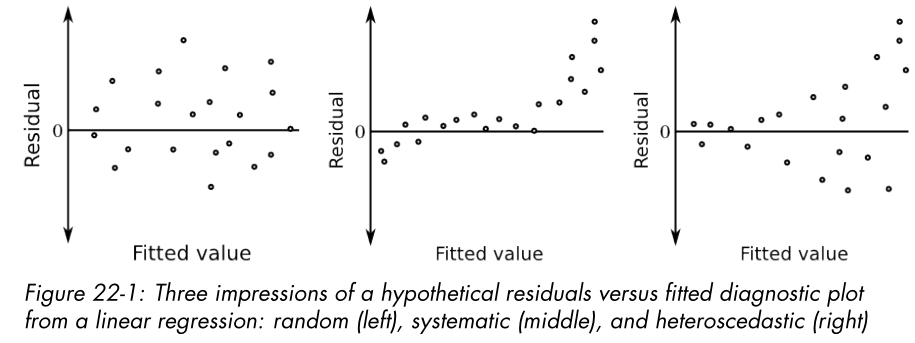
\includegraphics[scale =.6 ]  {figures/scatterplot_residuals.png}}
\end{figure}











\end{document}

